\chapter{Evaluation}
\label{ch:evaluation}

How much data compression does the Hypertrie achieve due to applying the space reduction approach presented earlier? 
Does the new data structure compromise the overall efficiency, more specifically, the query processing speed? 
On the one side, this chapter describes the space-friendliness of Hypertrie by presenting the compression ratio achieved w.r.t. the original Hypertrie after the bulk loading with different RDF data sets is done for both Hypertrie variants.  
On the other side, we have a look at how the space enhanced Tentris can still maintain its proven efficiency. For that, I ran a a series of benchmark experiments on real RDF data and queries. \\

As this work's effort is mainly toward enhancing the Tentris system in the context of space cost, all the experiments consider only the original Tentris' Hypertrie as the reference for comparison opting out other triple store systems. The experimental setup is described in section \ref{sec:exper_setup}. In the succeeding section \ref{sec:results}, the results are presented.

\section{Experimental Setup}
\label{sec:exper_setup}

\subsection{Data Sets and Queries}
\label{subsec:datasets}

 I used three different RDF data sets to assess the performance  (load time/ size) of the compressed Hypertrie. Concretely, I used Semantic Web Dog Food SWDF (372K triples) as well as the English DBpedia 2015-10 (681 M triples) as real-world data sets. 
I also chose the 1 billion-triple synthetic data set from WatDiv \cite{WatDiv} (see Table \ref{tab:datasets_status}). All the three data sets were used during the size/load speed assessment. However, only SWDF and DBpedia data set were incorporated into the benchmarks.

\begin{table}[tb]
	\centering
	\setlength{\tabcolsep}{1ex}
	\begin{tabular}{lrrrrl}
		\toprule
		Dataset&\#T&\#S&\#P&\#O& {Type}\\
		\midrule
		SWDF & 372\;\;\,k & 32\;\;\,k & 185 & 96\;\;\,k  & real-world\\ % structuredness 0.027901741842416984
		DBpedia & 681\;M & 40\;M & 63\;k & 178\;M & real-world \\ % structuredness
		WatDiv & 1\;\,G & 52\;M & 186 & 92\;M & synthetic\\ % structuredness 0.005427051162802224
		% DBpedia & 681'333'018 & 40'426'431 & 62658 & 178'269'555
		% WatDiv & 1091468578 & 52120385 & 186 & 92'240'568
		\bottomrule
	\end{tabular}
	\caption{RDF datasets which were used throughout the evaluation phase. Numbers of distinct triples (T), subjects (S), predicates (P) and objects (O) of each dataset. Additionally, Type classifies the datasets as real-world or synthetic. }
	\label{tab:datasets_status}
\end{table}

\subsection{Test Environment} I used the server machine "Geiser" provisioned and maintained by the data science research group at Paderborn university to run all the experiments. 
The server machine has two Xeon E5-2683 v4 CPUs and 512 GB of RAM. 
Geiser runs Ubuntu 18.04.4 LTS 64-bit on Linux Kernel 4.15.0-112-generic with Python 3.6.9 and OpenJDK Java 11.0.8 installed\footnote{The server specification may change in the future. However, by the time of the document submission date, the spec mentioned here holds.}.
The benchmark tool and the Tentris triple stores (compressed/ non-compressed) were installed locally on a single server instance to avoid network latency. 
Data sets held in N-Triples format (\verb|.nt| files) were uploaded to the server and stored on disk.

\subsection{Bulk Loading} 
Generally, bulk loading is the activity of loading a large volume of data into a data storage system (database, triple store, etc.) mainly in one call, thus in a relatively small amount of time. 
There are many use cases in which bulk loading could apply; one example is data import/ export.
In this work context, bulk loading is used to load an entire RDF graph into Tentris; thus, it can calculate its memory footprint and the time to load.
During the bulk loading experiment, all the three RDF datasets (Sec. \ref{subsec:datasets}) were involved for each variant of the triple stores (compressed, non-compressed).
I also expanded the load test to check the space utilization performance of the compressed Hypertrie as the dataset scales.
For that, I used generated WatDiv synthetic datasets with increasing scale factors: [10, 100, 1000, 10000]. 
The bulk loading tests' results were calculated using a set of utility methods inside the Tentris project. Those utilities rely on built-in functions inside C++ language, which interface low-level system services and data to their clients.

\subsubsection{Calculating Size}
There are many methods to calculate memory utilization of processes or data structures residents. 
Each method fits a set of use cases and they can vary with accuracy.
For the case at hand, I relied on the \verb|proc| virtual file system in the server instance that ran the experiments. Given that, "The \verb|proc| filesystem is a pseudo-filesystem which provides an
interface to kernel data structures.  It is commonly mounted at
\verb|/proc|.  
Typically, it is mounted automatically by the system, but it can also be mounted manually" \footnote{https://man7.org/linux/man-pages/man5/proc.5.html}. The content of the files inside \verb|proc| has mostely the status of \textit{read-only} as the files are written by the kernel. 
For each process (with a process id \textit{pid}) currently running in the linux system, there exists a subdirectory \verb|/proc/[|\textit{pid}\verb|]|. 
Underbeneath each subdirectory \verb|/proc/[|\textit{pid}\verb|]|, there are a set of files and subdirectories disclosing meta-information about process with \textit{pid}. The file \verb|/proc/[|\textit{pid}\verb|]/status| provides status information about the process including various memory consumption information. The information are provided in a human-readable fashion. \\

After a single bulk load experiment is finished, Tentris access the corresponding status file; i.e. \verb|/proc/slef/status| where the magic symbolic link \verb|self| is automatically evaluated to Tentris' process ID. The field \verb|VmRSS| inside \verb|Status| file provide the current memory utilization of the resident Tentris process including the sizes of resident anonymous memory, resident file mappings and resident shared memory. 

\subsubsection{Calculating Load Time}
A simple tic-toc approach is adopted to calculate the load speed of RDF graphs into Tentris. More specifically, two start and end time flags are setup immediately before and after the actual loading of keys. The difference between the time checkpoints is then calculated to capture the load speed.  \\

The time checkpoints calculation utilized \verb|steady_clock| instead of \verb|system_clock|.
As \verb|system_clock| talks periodically to machine clock to correct itself, it might make minor timing mistakes. As \verb|steady_clock| is independent from the system clock, thus providing more reliable timing insights. 
 
\subsection{Benchmark Execution}
For executing the benchmark, I used the generic SPARQL benchmark execution framework IGUANA v3.0.0-alpha2 \cite{conrads-2017-iguana-demo}. 
IGUANA is a benchmark suite for executing benchmarks. 
It takes a benchmark, namely a data set and a possible list of SPARQL queries/updates, as input. 
Then it simulates a SPARQL user that pushes a series of queries repeatedly in a stress test scenario to a SPARQL endpoint where the next request is sent immediately after returning the last response. 
IGUANA can execute both synthetic benchmarks and benchmarks based on real data.
As part of its execution, the suite returns information on the respective triple store's different behavioral aspects, such as query processing speed for each query and the query result's size. 
The framework enables different benchmark execution options and fashions (measure performance of triple stores under updates, parallel user requests, etc ...). 
As Tentris provides an HTTP-based SPARQL interface, I used the HTTP-based benchmark with one user as a benchmark setup. 
The suite returned the average response time for each query, and the query result's size to consider later for comparison.  \\

\section{Results}
\label{sec:results}

\clearpage

\begin{figure}[h]
	\label{fig:benchmarks}
	\centering
	\subfloat[SWDF]{%
		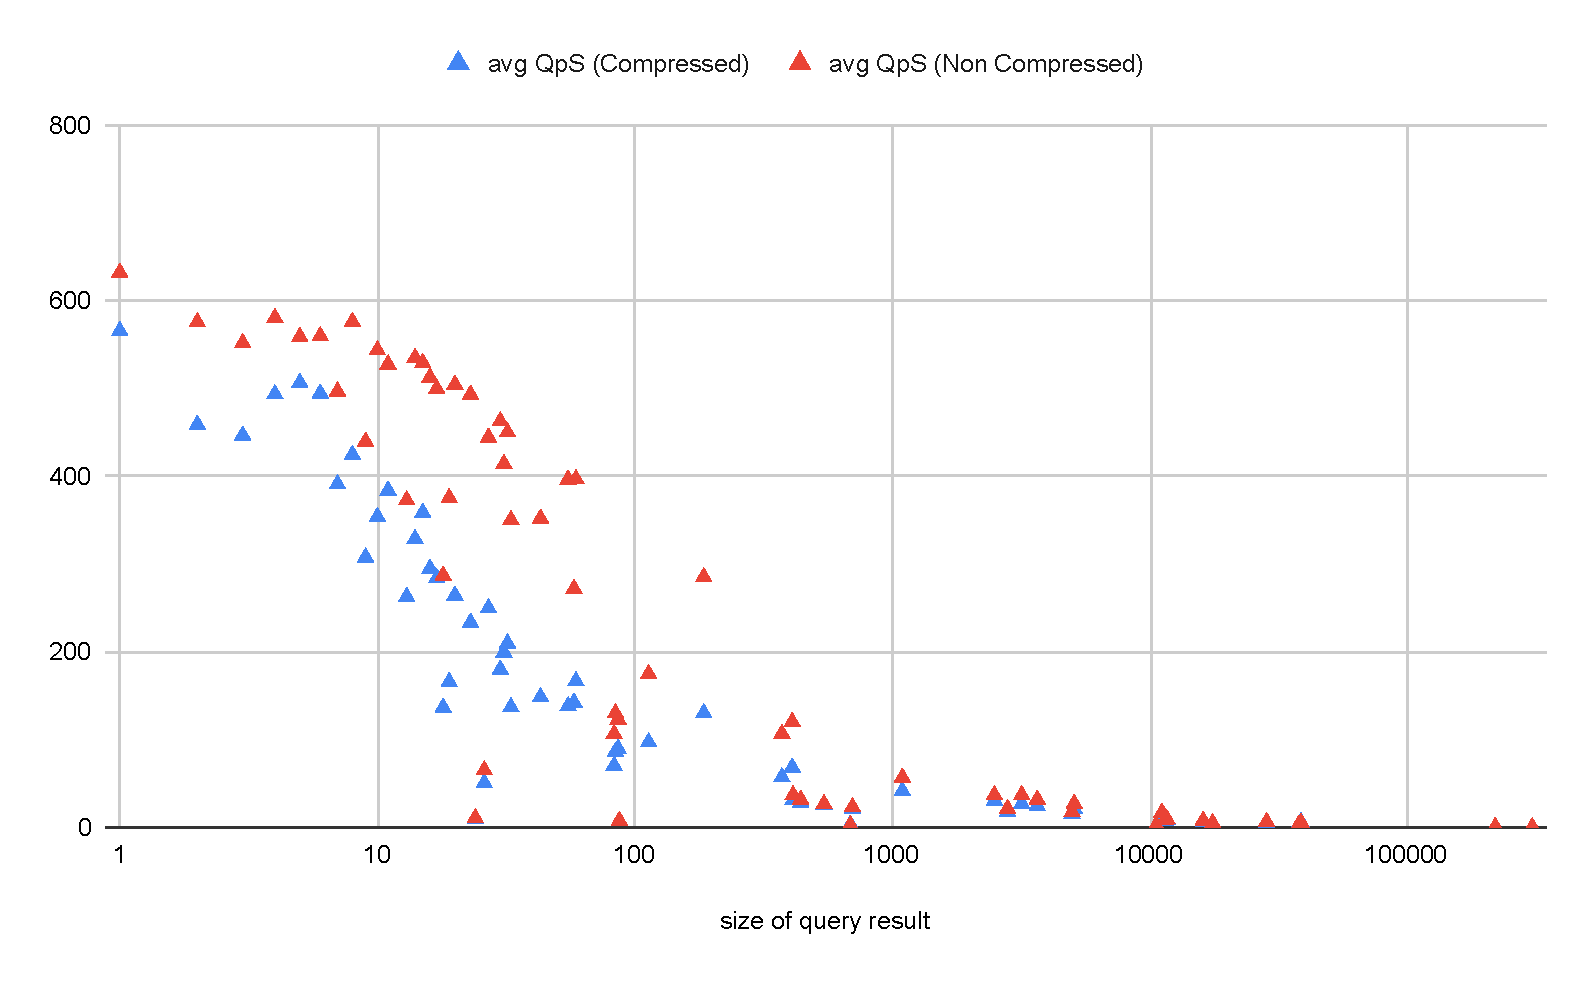
\includegraphics[width=\textwidth]{figures/chapter5/SWDFBenchmarktriangle}
	}
	
	\subfloat[DBpedia]{%
	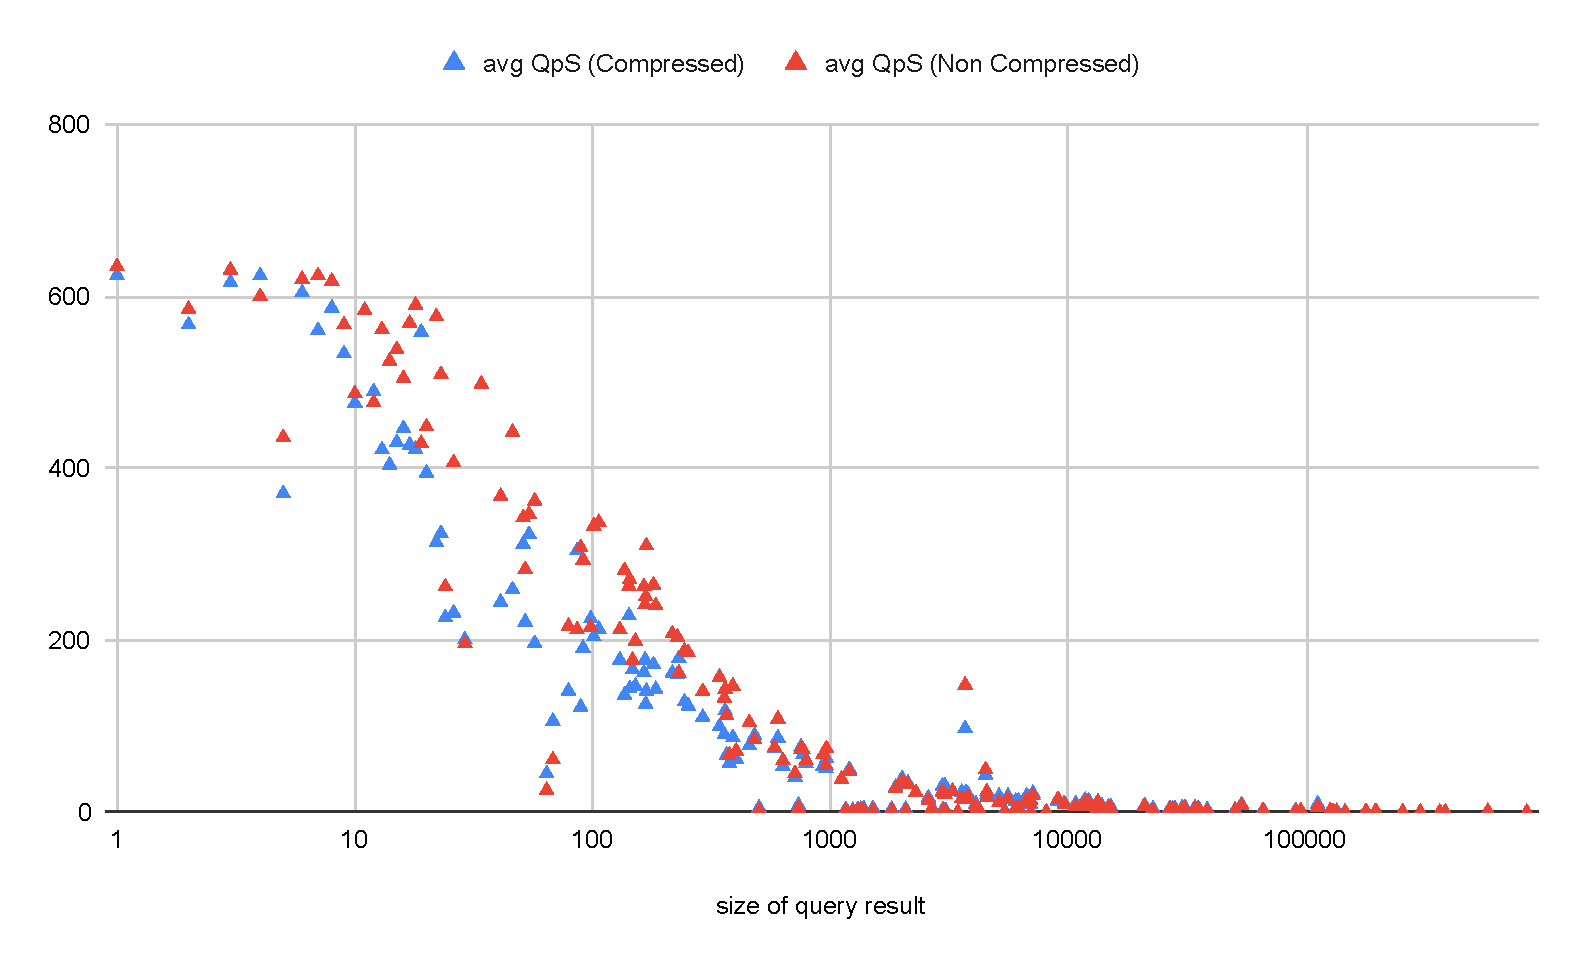
\includegraphics[width=\textwidth]{figures/chapter5/DBpediaBenchmarktriangle}%
	}
	
	\caption{Average Queries per Second (avg QpS) by size of the query result considering the two variants of Hypertrie implementations (compressed, non-compressed). Figure 5.1a shows the results of benchmarking against SWDF dataset and associated queries, while figure 5.1b shows  the results of benchmarking against DBpedia dataset.}
\end{figure}
\clearpage